% coding:utf-8

%FOSAET, a LaTeX-Code for a electrical summary of basic electronics
%Copyright (C) 2013, Daniel Winz, Ervin Mazlagic

%This program is free software; you can redistribute it and/or
%modify it under the terms of the GNU General Public License
%as published by the Free Software Foundation; either version 2
%of the License, or (at your option) any later version.

%This program is distributed in the hope that it will be useful,
%but WITHOUT ANY WARRANTY; without even the implied warranty of
%MERCHANTABILITY or FITNESS FOR A PARTICULAR PURPOSE.  See the
%GNU General Public License for more details.
%----------------------------------------

\chapter{Bauteile}
\newpage

%Widerstand 
% coding:utf-8

%FOSAET, a LaTeX-Code for a electrical summary of basic electronics
%Copyright (C) 2013, Daniel Winz, Ervin Mazlagic

%This program is free software; you can redistribute it and/or
%modify it under the terms of the GNU General Public License
%as published by the Free Software Foundation; either version 2
%of the License, or (at your option) any later version.

%This program is distributed in the hope that it will be useful,
%but WITHOUT ANY WARRANTY; without even the implied warranty of
%MERCHANTABILITY or FITNESS FOR A PARTICULAR PURPOSE.  See the
%GNU General Public License for more details.
%----------------------------------------

\section{Widerstand}
\[ R = \frac{U}{I} \]
             % Widerstand
% coding:utf-8

%FOSAET, a LaTeX-Code for a electrical summary of basic electronics
%Copyright (C) 2013, Daniel Winz, Ervin Mazlagic

%This program is free software; you can redistribute it and/or
%modify it under the terms of the GNU General Public License
%as published by the Free Software Foundation; either version 2
%of the License, or (at your option) any later version.

%This program is distributed in the hope that it will be useful,
%but WITHOUT ANY WARRANTY; without even the implied warranty of
%MERCHANTABILITY or FITNESS FOR A PARTICULAR PURPOSE.  See the
%GNU General Public License for more details.
%----------------------------------------

\subsection{Widerstand einer Leitung}
\[ R = \frac{\rho \cdot \ell}{A} \]
\begin{tabular}{lp{0.8\textwidth}}
$\rho$&Spezifischer Widerstand\\
&(Achtung! liegt meist nicht in SI-Einheiten vor)\\
$\ell$&Länge\\
   $A$&Fläche
\end{tabular}

\subsubsection{Spezifischer Widerstand gängiger Materialien}
\begin{table}[h!]
\begin{tabular}{lr}
  Silber    & $1.63 \cdot 10^{-2} \frac{\Omega \cdot mm^2}{m}$ \\
  Kupfer    & $1.73 \cdot 10^{-2} \frac{\Omega \cdot mm^2}{m}$ \\
  Gold      & $2.21 \cdot 10^{-2} \frac{\Omega \cdot mm^2}{m}$ \\
  Aluminium & $2.63 \cdot 10^{-2} \frac{\Omega \cdot mm^2}{m}$ \\
  Messing   & $7.52 \cdot 10^{-2} \frac{\Omega \cdot mm^2}{m}$ \\
  Manganin  & $0.435 \frac{\Omega \cdot mm^2}{m}$ \\
\end{tabular}
\label{tab_spezwid}
\caption{Werte aus den Unterrichtsunterlagen}
\end{table}        % Spezifischer Widerstand
% coding:utf-8

%FOSAET, a LaTeX-Code for a electrical summary of basic electronics
%Copyright (C) 2013, Daniel Winz, Ervin Mazlagic

%This program is free software; you can redistribute it and/or
%modify it under the terms of the GNU General Public License
%as published by the Free Software Foundation; either version 2
%of the License, or (at your option) any later version.

%This program is distributed in the hope that it will be useful,
%but WITHOUT ANY WARRANTY; without even the implied warranty of
%MERCHANTABILITY or FITNESS FOR A PARTICULAR PURPOSE.  See the
%GNU General Public License for more details.
%----------------------------------------

\subsection{Stromdichte}
\[ \vec{J} = \frac{dI}{d\vec{A}} \]
\[ J = \frac{I}{A} \qquad \text{(homogenes Feld)} \]       % Stromdichte
% coding:utf-8

%FOSAET, a LaTeX-Code for a electrical summary of basic electronics
%Copyright (C) 2013, Daniel Winz, Ervin Mazlagic

%This program is free software; you can redistribute it and/or
%modify it under the terms of the GNU General Public License
%as published by the Free Software Foundation; either version 2
%of the License, or (at your option) any later version.

%This program is distributed in the hope that it will be useful,
%but WITHOUT ANY WARRANTY; without even the implied warranty of
%MERCHANTABILITY or FITNESS FOR A PARTICULAR PURPOSE.  See the
%GNU General Public License for more details.
%----------------------------------------

\subsection{Spannungsabhängigkeit}
Spannungskoeffizient
\[ \alpha_U = \frac{1}{R} \cdot \frac{\Delta R}{\Delta U} \]       % Spannungsabhängigkeit
% coding:utf-8

%FOSAET, a LaTeX-Code for a electrical summary of basic electronics
%Copyright (C) 2013, Daniel Winz, Ervin Mazlagic

%This program is free software; you can redistribute it and/or
%modify it under the terms of the GNU General Public License
%as published by the Free Software Foundation; either version 2
%of the License, or (at your option) any later version.

%This program is distributed in the hope that it will be useful,
%but WITHOUT ANY WARRANTY; without even the implied warranty of
%MERCHANTABILITY or FITNESS FOR A PARTICULAR PURPOSE.  See the
%GNU General Public License for more details.
%----------------------------------------

\subsection{Frequenzabhängigkeit}
\begin{figure}[h!]
  \centering
  \begin{circuitikz}[scale=1]\draw
    (0,0) to[short, o-*] (1,0)
    (1,0) to[short, *-] (1,1)
    (5,0) to[short, *-o] (6,0)
    (5,1) to[short, -*] (5,0)
    (1,0) to[R=R, *-] (3,0)
    (3,0) to[L=L, -*] (5,0)
    (1,1) to[C=C, ] (5,1)
    ;
  \end{circuitikz}
  \caption{Ersatzschaltbild bei hohen Frequenzen}
\end{figure}
\begin{tabular}{@{}lp{0.5\textwidth}}
R: & Widerstand \\
C: & Parallelkapazität ($\sim 1 pF$) \\
L: & Serieinduktivität ($\sim 1 - 10 nH$) \\
   & (Abhängig von der Bauform)
\end{tabular}        % Frequenzabhängigkeit
% coding:utf-8

%FOSAET, a LaTeX-Code for a electrical summary of basic electronics
%Copyright (C) 2013, Daniel Winz, Ervin Mazlagic

%This program is free software; you can redistribute it and/or
%modify it under the terms of the GNU General Public License
%as published by the Free Software Foundation; either version 2
%of the License, or (at your option) any later version.

%This program is distributed in the hope that it will be useful,
%but WITHOUT ANY WARRANTY; without even the implied warranty of
%MERCHANTABILITY or FITNESS FOR A PARTICULAR PURPOSE.  See the
%GNU General Public License for more details.
%----------------------------------------

\subsection{Rauschen}
Rauschleistung
\[ P_N = \frac{{U_N}^2}{R} = 4 \cdot k_b \cdot \vartheta \cdot \Delta f \]
\begin{tabular}{@{}lp{0.5\textwidth}}
  $P_N$         & Rauschleistung \\
  $U_N$         & Rauschspannung \\
  $k_b$         & Bolzmann-Konstante ($1.38066 [\frac{J}{K}]$) \\
  $\vartheta$   & Absoluttemperatur $[K]$\\
  $\Delta f$    & Bandbreite $[Hz]$ \\
\end{tabular}

\subsubsection{Addition der Rauschleistung}
\[ P_t = P_1 + P_2 + \dots \]
\[ U_t = \sqrt{{U_1}^2 + {U_2}^2 + \dots} \]      % Rauschen
% coding:utf-8

%FOSAET, a LaTeX-Code for a electrical summary of basic electronics
%Copyright (C) 2013, Daniel Winz, Ervin Mazlagic

%This program is free software; you can redistribute it and/or
%modify it under the terms of the GNU General Public License
%as published by the Free Software Foundation; either version 2
%of the License, or (at your option) any later version.

%This program is distributed in the hope that it will be useful,
%but WITHOUT ANY WARRANTY; without even the implied warranty of
%MERCHANTABILITY or FITNESS FOR A PARTICULAR PURPOSE.  See the
%GNU General Public License for more details.
%----------------------------------------

\subsection{Widerstandsreihen / E-Reihen}
\subsubsection{Berechnung}
\[ R_k = {\sqrt[n]{10}}^m \]
\begin{tabular}{@{}ll}
$R_k$: & Widerstandswert \\
$n$:   & Typ der Reihe (E $n$) (z.B. E12 $\rightarrow$ $n=12$) \\
$m$:   & Stelle des Widerstandswertes in der Reihe \\
\end{tabular} \\
\textbf{Achtung!} Die Werte sind nicht korrekt mathematisch gerundet. Sie sind 
aus der Tabelle auf Seite \pageref{subsubsec:ereihe_tab} zu entnehmen. 

\subsection{Toleranz}
\begin{tabular}{ll}
Reihe & Toleranz \\
E3   & $\leq20\%$ \\
E6   & $20\%$ \\
E12  & $10\%$ \\
E24  & $5\%$ \\
E48  & $2\%$ \\
E96  & $1\%$ \\
E192 & $0.5\%$ \\
\end{tabular}

\subsubsection{Tabelle}
\label{subsubsec:ereihe_tab}
\begin{tiny}
\begin{tabular}{@{}c@{ }c@{ }c@{ }c@{ }c@{ }c@{ }c}
E3   & E6   & E12  & E24  & E48  & E96  & E192 \\
1,00 & 1,00 & 1,00 & 1,00 & 1,00 & 1,00 & 1,00 \\
     &      &      &      &      &      & 1,01 \\
     &      &      &      &      & 1,02 & 1,02 \\
     &      &      &      &      &      & 1,04 \\
     &      &      &      & 1,05 & 1,05 & 1,05 \\
     &      &      &      &      &      & 1,06 \\
     &      &      &      &      & 1,07 & 1,07 \\
     &      &      &      &      &      & 1,09 \\
     &      &      & 1,10 & 1,10 & 1,10 & 1,10 \\
     &      &      &      &      &      & 1,11 \\
     &      &      &      &      & 1,13 & 1,13 \\
     &      &      &      &      &      & 1,14 \\
     &      &      &      & 1,15 & 1,15 & 1,15 \\
     &      &      &      &      &      & 1,17 \\
     &      &      &      &      & 1,18 & 1,18 \\
     &      &      &      &      &      & 1,20 \\
     &      & 1,20 & 1,20 & 1,21 & 1,21 & 1,21 \\
     &      &      &      &      &      & 1,23 \\
     &      &      &      &      & 1,24 & 1,24 \\
     &      &      &      &      &      & 1,26 \\
     &      &      &      & 1,27 & 1,27 & 1,27 \\
     &      &      &      &      &      & 1,29 \\
     &      &      &      &      & 1,30 & 1,30 \\
     &      &      &      &      &      & 1,32 \\
     &      &      & 1,30 & 1,33 & 1,33 & 1,33 \\
     &      &      &      &      &      & 1,35 \\
     &      &      &      &      & 1,37 & 1,37 \\
     &      &      &      &      &      & 1,38 \\
     &      &      &      & 1,40 & 1,40 & 1,40 \\
     &      &      &      &      &      & 1,42 \\
     &      &      &      &      & 1,43 & 1,43 \\
     &      &      &      &      &      & 1,45 \\
     & 1,50 & 1,50 & 1,50 & 1,47 & 1,47 & 1,47 \\
     &      &      &      &      &      & 1,49 \\
     &      &      &      &      & 1,50 & 1,50 \\
     &      &      &      &      &      & 1,52 \\
     &      &      &      & 1,54 & 1,54 & 1,54 \\
     &      &      &      &      &      & 1,56 \\
     &      &      &      &      & 1,58 & 1,58 \\
     &      &      &      &      &      & 1,60 \\
     &      &      & 1,60 & 1,62 & 1,62 & 1,62 \\
     &      &      &      &      &      & 1,64 \\
     &      &      &      &      & 1,65 & 1,65 \\
     &      &      &      &      &      & 1,67 \\
     &      &      &      & 1,69 & 1,69 & 1,69 \\
     &      &      &      &      &      & 1,72 \\
     &      &      &      &      & 1,74 & 1,74 \\
     &      &      &      &      &      & 1,76 \\
     &      & 1,80 & 1,80 & 1,78 & 1,78 & 1,78 \\
     &      &      &      &      &      & 1,80 \\
     &      &      &      &      & 1,82 & 1,82 \\
     &      &      &      &      &      & 1,84 \\
     &      &      &      & 1,87 & 1,87 & 1,87 \\
     &      &      &      &      &      & 1,89 \\
     &      &      &      &      & 1,91 & 1,91 \\
     &      &      &      &      &      & 1,93 \\
     &      &      & 2,00 & 1,96 & 1,96 & 1,96 \\
     &      &      &      &      &      & 1,98 \\
     &      &      &      &      & 2,00 & 2,00 \\
     &      &      &      &      &      & 2,03 \\
     &      &      &      & 2,05 & 2,05 & 2,05 \\
     &      &      &      &      &      & 2,08 \\
     &      &      &      &      & 2,10 & 2,10 \\
     &      &      &      &      &      & 2,13 
\end{tabular}
\begin{tabular}{@{}c@{ }c@{ }c@{ }c@{ }c@{ }c@{ }c}
  E3 & E6   & E12  & E24  & E48 &  E96  & E192 \\
2,20 & 2,20 & 2,20 & 2,20 & 2,15 & 2,15 & 2,15 \\
     &      &      &      &      &      & 2,18 \\
     &      &      &      &      & 2,21 & 2,21 \\
     &      &      &      &      &      & 2,23 \\
     &      &      &      & 2,26 & 2,26 & 2,26 \\
     &      &      &      &      &      & 2,29 \\
     &      &      &      &      & 2,32 & 2,32 \\
     &      &      &      &      &      & 2,34 \\
     &      &      & 2,40 & 2,37 & 2,37 & 2,37 \\
     &      &      &      &      &      & 2,40 \\
     &      &      &      &      & 2,43 & 2,43 \\
     &      &      &      &      &      & 2,46 \\
     &      &      &      & 2,49 & 2,49 & 2,49 \\
     &      &      &      &      &      & 2,52 \\
     &      &      &      &      & 2,55 & 2,55 \\
     &      &      &      &      &      & 2,58 \\
     &      & 2,70 & 2,70 & 2,61 & 2,61 & 2,61 \\
     &      &      &      &      &      & 2,64 \\
     &      &      &      &      & 2,67 & 2,67 \\
     &      &      &      &      &      & 2,71 \\
     &      &      &      & 2,74 & 2,74 & 2,74 \\
     &      &      &      &      &      & 2,77 \\
     &      &      &      &      & 2,80 & 2,80 \\
     &      &      &      &      &      & 2,84 \\
     &      &      & 3,00 & 2,87 & 2,87 & 2,87 \\
     &      &      &      &      &      & 2,91 \\
     &      &      &      &      & 2,94 & 2,94 \\
     &      &      &      &      &      & 2,98 \\
     &      &      &      & 3,01 & 3,01 & 3,01 \\
     &      &      &      &      &      & 3,05 \\
     &      &      &      &      & 3,09 & 3,09 \\
     &      &      &      &      &      & 3,12 \\
     & 3,30 & 3,30 & 3,30 & 3,16 & 3,16 & 3,16 \\
     &      &      &      &      &      & 3,20 \\
     &      &      &      &      & 3,24 & 3,24 \\
     &      &      &      &      &      & 3,28 \\
     &      &      &      & 3,32 & 3,32 & 3,32 \\
     &      &      &      &      &      & 3,36 \\
     &      &      &      &      & 3,40 & 3,40 \\
     &      &      &      &      &      & 3,44 \\
     &      &      & 3,60 & 3,48 & 3,48 & 3,48 \\
     &      &      &      &      &      & 3,52 \\
     &      &      &      &      & 3,57 & 3,57 \\
     &      &      &      &      &      & 3,61 \\
     &      &      &      & 3,65 & 3,65 & 3,65 \\
     &      &      &      &      &      & 3,70 \\
     &      &      &      &      & 3,74 & 3,74 \\
     &      &      &      &      &      & 3,79 \\
     &      & 3,90 & 3,90 & 3,83 & 3,83 & 3,83 \\
     &      &      &      &      &      & 3,88 \\
     &      &      &      &      & 3,92 & 3,92 \\
     &      &      &      &      &      & 3,97 \\
     &      &      &      & 4,02 & 4,02 & 4,02 \\
     &      &      &      &      &      & 4,07 \\
     &      &      &      &      & 4,12 & 4,12 \\
     &      &      &      &      &      & 4,17 \\
     &      &      & 4,30 & 4,22 & 4,22 & 4,22 \\
     &      &      &      &      &      & 4,27 \\
     &      &      &      &      & 4,32 & 4,32 \\
     &      &      &      &      &      & 4,37 \\
     &      &      &      & 4,42 & 4,42 & 4,42 \\
     &      &      &      &      &      & 4,48 \\
     &      &      &      &      & 4,53 & 4,53 \\
     &      &      &      &      &      & 4,59 
\end{tabular}
\begin{tabular}{@{}c@{ }c@{ }c@{ }c@{ }c@{ }c@{ }c}
  E3 & E6   & E12  & E24  & E48  & E96  & E192 \\
4,70 & 4,70 & 4,70 & 4,70 & 4,64 & 4,64 & 4,64 \\
     &      &      &      &      &      & 4,70 \\
     &      &      &      &      & 4,75 & 4,75 \\
     &      &      &      &      &      & 4,81 \\
     &      &      &      & 4,87 & 4,87 & 4,87 \\
     &      &      &      &      &      & 4,93 \\
     &      &      &      &      & 4,99 & 4,99 \\
     &      &      &      &      &      & 5,05 \\
     &      &      & 5,10 & 5,11 & 5,11 & 5,11 \\
     &      &      &      &      &      & 5,17 \\
     &      &      &      &      & 5,23 & 5,23 \\
     &      &      &      &      &      & 5,30 \\
     &      &      &      & 5,36 & 5,36 & 5,36 \\
     &      &      &      &      &      & 5,42 \\
     &      &      &      &      & 5,49 & 5,49 \\
     &      &      &      &      &      & 5,56 \\
     &      & 5,60 & 5,60 & 5,62 & 5,62 & 5,62 \\
     &      &      &      &      &      & 5,69 \\
     &      &      &      &      & 5,76 & 5,76 \\
     &      &      &      &      &      & 5,83 \\
     &      &      &      & 5,90 & 5,90 & 5,90 \\
     &      &      &      &      &      & 5,97 \\
     &      &      &      &      & 6,04 & 6,04 \\
     &      &      &      &      &      & 6,12 \\
     &      &      & 6,20 & 6,19 & 6,19 & 6,19 \\
     &      &      &      &      &      & 6,26 \\
     &      &      &      &      & 6,34 & 6,34 \\
     &      &      &      &      &      & 6,42 \\
     &      &      &      & 6,49 & 6,49 & 6,49 \\
     &      &      &      &      &      & 6,57 \\
     &      &      &      &      & 6,65 & 6,65 \\
     &      &      &      &      &      & 6,73 \\
     & 6,80 & 6,80 & 6,80 & 6,81 & 6,81 & 6,81 \\
     &      &      &      &      &      & 6,90 \\
     &      &      &      &      & 6,98 & 6,98 \\
     &      &      &      &      &      & 7,06 \\
     &      &      &      & 7,15 & 7,15 & 7,15 \\
     &      &      &      &      &      & 7,23 \\
     &      &      &      &      & 7,32 & 7,32 \\
     &      &      &      &      &      & 7,41 \\
     &      &      & 7,50 & 7,50 & 7,50 & 7,50 \\
     &      &      &      &      &      & 7,59 \\
     &      &      &      &      & 7,68 & 7,68 \\
     &      &      &      &      &      & 7,77 \\
     &      &      &      & 7,87 & 7,87 & 7,87 \\
     &      &      &      &      &      & 7,96 \\
     &      &      &      &      & 8,06 & 8,06 \\
     &      &      &      &      &      & 8,16 \\
     &      & 8,20 & 8,20 & 8,25 & 8,25 & 8,25 \\
     &      &      &      &      &      & 8,35 \\
     &      &      &      &      & 8,45 & 8,45 \\
     &      &      &      &      &      & 8,56 \\
     &      &      &      & 8,66 & 8,66 & 8,66 \\
     &      &      &      &      &      & 8,76 \\
     &      &      &      &      & 8,87 & 8,87 \\
     &      &      &      &      &      & 8,98 \\
     &      &      & 9,10 & 9,09 & 9,09 & 9,09 \\
     &      &      &      &      &      & 9,20 \\
     &      &      &      &      & 9,31 & 9,31 \\
     &      &      &      &      &      & 9,42 \\
     &      &      &      & 9,53 & 9,53 & 9,53 \\
     &      &      &      &      &      & 9,65 \\
     &      &      &      &      & 9,76 & 9,76 \\
     &      &      &      &      &      & 9,88 
\end{tabular}
\end{tiny}
      % Widerstandsreihen, E-Reihen
% coding:utf-8

%FOSAET, a LaTeX-Code for a electrical summary of basic electronics
%Copyright (C) 2013, Daniel Winz, Ervin Mazlagic

%This program is free software; you can redistribute it and/or
%modify it under the terms of the GNU General Public License
%as published by the Free Software Foundation; either version 2
%of the License, or (at your option) any later version.

%This program is distributed in the hope that it will be useful,
%but WITHOUT ANY WARRANTY; without even the implied warranty of
%MERCHANTABILITY or FITNESS FOR A PARTICULAR PURPOSE.  See the
%GNU General Public License for more details.
%----------------------------------------

\subsection{Temperaturabhängigkeit von Widerständen}

\subsubsection{Lineare Temperaturabhängigkeit von Widerständen}
\[ R_\vartheta = R_{20} \cdot (1 + \alpha \cdot \Delta \vartheta) \]
\[ \Delta R = R_{20} \cdot \alpha \cdot \Delta \vartheta \]
Falls $R_{20}$ nicht bekannt ist, kann mit $R_A$ bei $\vartheta_a$ und $\tau$ 
die Temperaturabhängigkeit mit folgender Formel berechnet werden:  
\[ R_\vartheta = R_A \frac{\tau + \vartheta}{\tau + \vartheta_A} 
\qquad \text{Wobei} 
\qquad \tau = \frac{1}{\alpha_20} - 20^{\circ}\text{C} \]

\subsubsection{Platintemperatursensoren (PT100, PT1000 \dots)}
Zwischen $0^\circ$ und $100^\circ$ kann die Temperaturabhängigkeit linear 
berechnet werden. 
\[ \begin{array}{l}
R_\vartheta = R_0 \cdot (1 + a \cdot \vartheta) \\
a = 3.85 \cdot 10^{-3} \left[\frac{1}{K}\right] 
\end{array} \]
%
Für höhere Temperaturen oder höhere Genauigkeit wird ein Polynom vom Grad 2 
verwendet. 
\[ \begin{array}{l}
R_\vartheta = R_0 \cdot (1 + a \cdot \vartheta + b \cdot \vartheta^2) \\
a = 3.9083 \cdot 10^{-3} \left[\frac{1}{K}\right] \\
b = -5.775 \cdot 10^{-7} \left[\frac{1}{K^2}\right] 
\end{array} \]
%
Für Temperaturen unter $0^\circ C$ wird ein Polynom vom Grad 4 verwendet. 
\[ \begin{array}{l}
R_\vartheta = R_0 \cdot (1 + a \cdot \vartheta + b \cdot \vartheta^2 
+ c \cdot (\vartheta - 100^\circ C) \cdot \vartheta^3) \\
a = 3.9083 \cdot 10^{-3} \left[\frac{1}{K}\right] \\
b = -5.775 \cdot 10^{-7} \left[\frac{1}{K^2}\right] \\
c = -4.183 \cdot 10^{-12} \left[\frac{1}{K^3}\right] 
\end{array} \]


\subsubsection{Nichtlineare Temperaturabhängigkeit (PTC)}
% \[ R_N = 2 \cdot R_A \]   Diese Formel macht nur mit Grafik Sinn!!!
\[ R_T = R_N \cdot e^{\alpha (T - T_N)} \]
\[ \alpha = \frac{\ln R_1 - \ln R_2}{T_2 - T_1} 
= \frac{\ln\left(\frac{R_1}{R_2}\right)}{\Delta T} 
= \frac{d R_t}{d T}\frac{1}{R_T} \]
\begin{tabular}{@{}lp{0.5\textwidth}}
  $t_A$:        & Anfangstemperatur $[^\circ C]$ \\
  $t_N$:        & Nenntemperatur $[^\circ C]$ \\
  $R_N$:        & Anfangswiderstand $[\Omega]$ \\
  $\alpha$:     & Temperaturkoeffizient oberhalb der Nenntemperatur 
                  ($+5\frac{\%}{K}$ bis $+70\frac{\%}{K}$) \\
  $R_1$, $R_2$: & Widerstände $[\Omega]$ für zwei Punkte oberhalb der 
                  Nenntemperatur \\
  $\Delta T$:   & Temperaturunterschied $[^\circ C]$ für die beiden Punkte mit 
                  $R_1$ und $R_2$
\end{tabular}

\subsubsection{Nichtlineare Temperaturabhängigkeit (NTC)}
\[ R_T = R_N \cdot e^{B\left(\frac{1}{T} - \frac{1}{T_N}\right)} 
= A \cdot e^{\frac{B}{T}} \]
\[ \alpha_T = \frac{d R_T}{d T}\frac{1}{R_T} = -\frac{B}{T^2} 
\qquad B = -\alpha_T \cdot T^2 \]
\begin{tabular}{@{}lp{0.5\textwidth}}
  $R_T$:        & Heissleiterwiderstand bei $T[K]$ in $[\Omega]$ \\
  $R_N$:        & R bei Bezugstemperatur 
                  ($293 K$ entsprechen $20^\circ C$ $[\Omega]$) \\
  $T$:          & Betriebs-, Umgebungstemperatur $[K]$ \\
  $T_N$:        & Bezugstemperatur $[K]$ \\
  $A$:          & Formkonstante $[\Omega]$ nach Herstellerangaben \\
  $B$:          & Regelkonstante $[K]$ \\
  $\alpha_T$:   & temperaturabhängiger Temperaturkoeffizient bei $T$ $[K]$
\end{tabular}        % Temperaturabhängigkeit von Widerständen
% coding:utf-8

%FOSAET, a LaTeX-Code for a electrical summary of basic electronics
%Copyright (C) 2013, Daniel Winz, Ervin Mazlagic

%This program is free software; you can redistribute it and/or
%modify it under the terms of the GNU General Public License
%as published by the Free Software Foundation; either version 2
%of the License, or (at your option) any later version.

%This program is distributed in the hope that it will be useful,
%but WITHOUT ANY WARRANTY; without even the implied warranty of
%MERCHANTABILITY or FITNESS FOR A PARTICULAR PURPOSE.  See the
%GNU General Public License for more details.
%----------------------------------------

\subsection{Varistor (VDR)}

\[ U = C \cdot I^{\beta} \]
\[ I = \left(\frac{U}{C}\right)^{\frac{1}{\beta}} \]
\begin{tabular}{@{}lp{0.5\textwidth}}
  $\beta$: & Regelfaktor, Stromindex \\
  $C$:     & Konstante, die von den Abmessungen des VDR-Widerstandes abhängt
\end{tabular}         % Varistor
% coding:utf-8

%FOSAET, a LaTeX-Code for a electrical summary of basic electronics
%Copyright (C) 2013, Daniel Winz, Ervin Mazlagic

%This program is free software; you can redistribute it and/or
%modify it under the terms of the GNU General Public License
%as published by the Free Software Foundation; either version 2
%of the License, or (at your option) any later version.

%This program is distributed in the hope that it will be useful,
%but WITHOUT ANY WARRANTY; without even the implied warranty of
%MERCHANTABILITY or FITNESS FOR A PARTICULAR PURPOSE.  See the
%GNU General Public License for more details.
%----------------------------------------

\subsection{LDR}
\[ R_F = R_0 \cdot \left( \frac{E_0}{E} \right)^n \]         % LDR

% Kondensator
% coding:utf-8

%FOSAET, a LaTeX-Code for a electrical summary of basic electronics
%Copyright (C) 2013, Daniel Winz, Ervin Mazlagic

%This program is free software; you can redistribute it and/or
%modify it under the terms of the GNU General Public License
%as published by the Free Software Foundation; either version 2
%of the License, or (at your option) any later version.

%This program is distributed in the hope that it will be useful,
%but WITHOUT ANY WARRANTY; without even the implied warranty of
%MERCHANTABILITY or FITNESS FOR A PARTICULAR PURPOSE.  See the
%GNU General Public License for more details.
%----------------------------------------

\newpage
\section{Kondensator}
\[ C = \frac{Q}{U} \]
            % Kondensator
% coding:utf-8

%FOSAET, a LaTeX-Code for a electrical summary of basic electronics
%Copyright (C) 2013, Daniel Winz, Ervin Mazlagic

%This program is free software; you can redistribute it and/or
%modify it under the terms of the GNU General Public License
%as published by the Free Software Foundation; either version 2
%of the License, or (at your option) any later version.

%This program is distributed in the hope that it will be useful,
%but WITHOUT ANY WARRANTY; without even the implied warranty of
%MERCHANTABILITY or FITNESS FOR A PARTICULAR PURPOSE.  See the
%GNU General Public License for more details.
%----------------------------------------

\subsection{Kapazität}
\subsubsection{Plattenkondensator}
\[ C = \frac{A \cdot \varepsilon}{\ell} 
= \frac{A \cdot \varepsilon_0 \cdot \varepsilon_r}{\ell} \]
\begin{tabular}{lp{0.8\textwidth}}
$\varepsilon$&Permittivität\\
$\varepsilon_0$&elektrische Feldkonstante\\
&(Permittivität von Vakuum)\\
&($8.854 \cdot 10^{-12} \left[\frac{F}{m}\right]$)\\
$\varepsilon_r$&relative Permittivität\\
$A$&Plattenfläche\\
$\ell$&Plattenabstand
\end{tabular}        % Kapazität
% coding:utf-8

%FOSAET, a LaTeX-Code for a electrical summary of basic electronics
%Copyright (C) 2013, Daniel Winz, Ervin Mazlagic

%This program is free software; you can redistribute it and/or
%modify it under the terms of the GNU General Public License
%as published by the Free Software Foundation; either version 2
%of the License, or (at your option) any later version.

%This program is distributed in the hope that it will be useful,
%but WITHOUT ANY WARRANTY; without even the implied warranty of
%MERCHANTABILITY or FITNESS FOR A PARTICULAR PURPOSE.  See the
%GNU General Public License for more details.
%----------------------------------------

\subsection{Energie im Kondensator}
\[ W_e = \frac{C \cdot U^2}{2} = \frac{Q \cdot U}{2} = \frac{Q^2}{2 \cdot C} \]       % Energie im Kondensator
% coding:utf-8

%FOSAET, a LaTeX-Code for a electrical summary of basic electronics
%Copyright (C) 2013, Daniel Winz, Ervin Mazlagic

%This program is free software; you can redistribute it and/or
%modify it under the terms of the GNU General Public License
%as published by the Free Software Foundation; either version 2
%of the License, or (at your option) any later version.

%This program is distributed in the hope that it will be useful,
%but WITHOUT ANY WARRANTY; without even the implied warranty of
%MERCHANTABILITY or FITNESS FOR A PARTICULAR PURPOSE.  See the
%GNU General Public License for more details.
%----------------------------------------

\subsection{Parallelschaltung von Kondensatoren}
\[ C_{ges} = \sum_{k=1}^{n} C_k \]

\subsection{Serieschaltung von Kondensatoren}
\[ \frac{1}{C_{ges}} = \sum_{k=1}^{n} \frac{1}{C_k} \]     % Parallel und Serieschaltung
% coding:utf-8

%FOSAET, a LaTeX-Code for a electrical summary of basic electronics
%Copyright (C) 2013, Daniel Winz, Ervin Mazlagic

%This program is free software; you can redistribute it and/or
%modify it under the terms of the GNU General Public License
%as published by the Free Software Foundation; either version 2
%of the License, or (at your option) any later version.

%This program is distributed in the hope that it will be useful,
%but WITHOUT ANY WARRANTY; without even the implied warranty of
%MERCHANTABILITY or FITNESS FOR A PARTICULAR PURPOSE.  See the
%GNU General Public License for more details.
%----------------------------------------

\newpage
\subsection{Ersatzschaltung}
\begin{figure}[h!]
  \centering
  \begin{circuitikz}[scale=1]\draw
    (0,0) to[short, o-] (1,0)
    (7,0) to[short, -o] (8,0)
    (1,0) to[R=$R_C$, ] (3,0)
    (3,0) to[L=$L_C$, ] (5,0)
    (5,0) to[C=C, ] (7,0)
    ;
  \end{circuitikz}
  \caption{Ersatzschaltung eines Kondensators}
\end{figure}
     % Ersatzschaltung Kondensator
% coding:utf-8

%FOSAET, a LaTeX-Code for a electrical summary of basic electronics
%Copyright (C) 2013, Daniel Winz, Ervin Mazlagic

%This program is free software; you can redistribute it and/or
%modify it under the terms of the GNU General Public License
%as published by the Free Software Foundation; either version 2
%of the License, or (at your option) any later version.

%This program is distributed in the hope that it will be useful,
%but WITHOUT ANY WARRANTY; without even the implied warranty of
%MERCHANTABILITY or FITNESS FOR A PARTICULAR PURPOSE.  See the
%GNU General Public License for more details.
%----------------------------------------

\subsection{Verluste im Kondensator}
\[ Q_C = \frac{P_B}{P_W} = \tan(\varphi) = \frac{1}{\tan(\delta)} 
\qquad \delta = 90^\circ - \varphi \]
\begin{tabular}{@{}ll}
  $Q_C$: & Güte \\
  $P_B$: & Blindleistung \\
  $P_W$: & Wirkleistung
\end{tabular}

\subsubsection{Serieersatzschaltung}
\begin{figure}[h!]
  \centering
  \begin{circuitikz}[scale=1]\draw
    (0,0) to[short, o-] (1,0)
    (5,0) to[short, -o] (6,0)
    (1,0) to[R=$R_s$, ] (3,0)
    (3,0) to[C=$C$, ] (5,0)
    ;
  \end{circuitikz}
  \caption{Serieersatzschaltung}
\end{figure}
\[ \tan(\delta_s) = R_s \cdot \omega \cdot C = \frac{1}{Q_c} \]

\subsubsection{Parallelersatzschaltung}
\begin{figure}[h!]
  \centering
  \begin{circuitikz}[scale=1]\draw
    (0,1) to[short, o-*] (1,1)
    (3,1) to[short, *-o] (4,1)
    (1,0) to[short, ] (1,2)
    (3,0) to[short, ] (3,2)
    (1,2) to[C=$C$, ] (3,2)
    (1,0) to[R=$R_p$, ] (3,0)
    ;
  \end{circuitikz}
  \caption{Parallelersatzschaltung}
\end{figure}
\[ \tan(\delta_p) = \frac{1}{R_p \cdot \omega \cdot C} \]
\[ \text{für } \tan(\delta) < 0.1 :
\qquad \tan(\delta) = \tan(\delta_s) = \tan(\delta_p) \]

\subsubsection{Verlustleistung}
\[ P_v = R_s \cdot i^2 \]
\[ P_v = 2 \cdot \pi \cdot f \cdot C \cdot U^2 \cdot \tan(\delta) \]       % Verluste im Kondensator



% Induktivität
% coding:utf-8

%FOSAET, a LaTeX-Code for a electrical summary of basic electronics
%Copyright (C) 2013, Daniel Winz, Ervin Mazlagic

%This program is free software; you can redistribute it and/or
%modify it under the terms of the GNU General Public License
%as published by the Free Software Foundation; either version 2
%of the License, or (at your option) any later version.

%This program is distributed in the hope that it will be useful,
%but WITHOUT ANY WARRANTY; without even the implied warranty of
%MERCHANTABILITY or FITNESS FOR A PARTICULAR PURPOSE.  See the
%GNU General Public License for more details.
%----------------------------------------

\newpage
\section{Spule}
\[ L = \frac{N \cdot \Phi}{I} \]
\begin{tabular}{@{}ll}
  $L$:      & Induktivität, $\left[\frac{Vs}{A} = 1H \text{ (Henry)}\right]$ \\
  $I$:      & Strom $[A]$ \\
  $N$:      & Anzahl Wicklungen \\
  $\Phi$    & Magnetischer Fluss $\left[ Vs = 1Wb \text{ (Weber)}\right]$
\end{tabular}             % Spule
% coding:utf-8

%FOSAET, a LaTeX-Code for a electrical summary of basic electronics
%Copyright (C) 2013, Daniel Winz, Ervin Mazlagic

%This program is free software; you can redistribute it and/or
%modify it under the terms of the GNU General Public License
%as published by the Free Software Foundation; either version 2
%of the License, or (at your option) any later version.

%This program is distributed in the hope that it will be useful,
%but WITHOUT ANY WARRANTY; without even the implied warranty of
%MERCHANTABILITY or FITNESS FOR A PARTICULAR PURPOSE.  See the
%GNU General Public License for more details.
%----------------------------------------

\subsection{Magnetismus}

\subsubsection{Durchflutung}
\[ \Theta = I \cdot N \]

\subsubsection{Magnetische Feldstärke}
\[ H = \frac{\Theta}{\ell} \left[\frac{A}{m}\right] \]

\subsubsection{Magnetische Induktion}
\[ B = \mu_r \cdot \mu_0 \cdot H \left[\frac{Vs}{m^2} = 1T \text{ Tesla}\right] \]

\subsubsection{Magnetischer Fluss}
\[ \Phi = \int_A B \cdot dA \left[\frac{Vs}{m^2} \cdot m^2 = Vs\right] \]
Homogene Felder
\[ \Phi = B \cdot A \]

\subsubsection{Induktivität}
\[ L = \frac{N \cdot \Phi}{I} \]
         % Magnetismus
% coding:utf-8

%FOSAET, a LaTeX-Code for a electrical summary of basic electronics
%Copyright (C) 2013, Daniel Winz, Ervin Mazlagic

%This program is free software; you can redistribute it and/or
%modify it under the terms of the GNU General Public License
%as published by the Free Software Foundation; either version 2
%of the License, or (at your option) any later version.

%This program is distributed in the hope that it will be useful,
%but WITHOUT ANY WARRANTY; without even the implied warranty of
%MERCHANTABILITY or FITNESS FOR A PARTICULAR PURPOSE.  See the
%GNU General Public License for more details.
%----------------------------------------

\subsection{Induktivität verschiedener Spulenformen}

\subsubsection{Ringkernspule}
\[ L = \frac{N^2 \cdot \mu_0 \cdot \mu_r \cdot A}{\ell_m} \]
\[ \mu = \mu_0 \cdot \mu_r \]
\begin{tabular}{@{}ll}
  $\mu$:    & Permeabilität, megnetische Leitfähigkeit eines Stoffes \\
  $\mu_0$:  & magnetische Feldkonstante für Vakuum \\
            & $\mu_0 = 4 \cdot \pi \cdot 10^{-7} \left[\frac{Vs}{Am}\right]$ \\
  $\mu_r$:  & relative Permeabilität, Permeabilitätszahl \\
  $\ell_m$: & mittlere Feldlinienlänge \\
  $A$:      & Kernquerschnittsfläche \\
  $N$:      & Windungszahl
\end{tabular}

\subsubsection{Kreisringspule}
\[ L = \mu \cdot R \cdot \left(\ln\left(\frac{R}{r}\right) + 0.08\right) \]
\[ \mu = \mu_0 \qquad \text{in nichtmagnetischem Material (Luft)} \]
\begin{tabular}{@{}ll}
  $R$:  & Ringradius \\
  $r$:  & Toroidradius 
\end{tabular}

\subsubsection{Zylinderspule}
Verhältnis Länge - Durchmesser : $\ell \sim 5 \cdot D$:
\[ L = \mu_0 \cdot \frac{N^2 \cdot D^2 \cdot \pi}{4 \cdot \ell} \]
$\ell \sim D$:
\[ L = \mu_0 \cdot \frac{N^2 \cdot D^2 \cdot \pi}{4 \cdot (\ell + 0.45 \cdot D)} \]
        % Induktivität verschiedener Spulenformen
% coding:utf-8

%FOSAET, a LaTeX-Code for a electrical summary of basic electronics
%Copyright (C) 2013, Daniel Winz, Ervin Mazlagic

%This program is free software; you can redistribute it and/or
%modify it under the terms of the GNU General Public License
%as published by the Free Software Foundation; either version 2
%of the License, or (at your option) any later version.

%This program is distributed in the hope that it will be useful,
%but WITHOUT ANY WARRANTY; without even the implied warranty of
%MERCHANTABILITY or FITNESS FOR A PARTICULAR PURPOSE.  See the
%GNU General Public License for more details.
%----------------------------------------

\subsection{Induktionsgesetz}
Induktion einer Drahtschleife
\[ u_0(t) = -\frac{d \Phi}{d t} \]
statische Induktivität
\[ N \cdot \Phi = L \cdot I \]
dynamischer Induktionsvorgang
\[ u = - N \cdot \frac{d \Phi}{d t} \]
Selbstinduktion
\[ u = - L  \cdot \frac{d i}{d t} \]
\[ u_L = + L  \cdot \frac{d i}{d t} \]   % Induktionsgesetz
% coding:utf-8

%FOSAET, a LaTeX-Code for a electrical summary of basic electronics
%Copyright (C) 2013, Daniel Winz, Ervin Mazlagic

%This program is free software; you can redistribute it and/or
%modify it under the terms of the GNU General Public License
%as published by the Free Software Foundation; either version 2
%of the License, or (at your option) any later version.

%This program is distributed in the hope that it will be useful,
%but WITHOUT ANY WARRANTY; without even the implied warranty of
%MERCHANTABILITY or FITNESS FOR A PARTICULAR PURPOSE.  See the
%GNU General Public License for more details.
%----------------------------------------

\subsection{Energie in der Spule}
\[ W_m = \frac{L \cdot I^2}{2} = \frac{\Phi \cdot I}{2} \]
        % Energie in der Spule
% coding:utf-8

%FOSAET, a LaTeX-Code for a electrical summary of basic electronics
%Copyright (C) 2013, Daniel Winz, Ervin Mazlagic

%This program is free software; you can redistribute it and/or
%modify it under the terms of the GNU General Public License
%as published by the Free Software Foundation; either version 2
%of the License, or (at your option) any later version.

%This program is distributed in the hope that it will be useful,
%but WITHOUT ANY WARRANTY; without even the implied warranty of
%MERCHANTABILITY or FITNESS FOR A PARTICULAR PURPOSE.  See the
%GNU General Public License for more details.
%----------------------------------------

\subsection{Serieschaltung von Spulen}
\[ L_{ges} = \sum_{k=1}^{n} L_k \]

\subsection{Parallelschaltung von Spulen}
\[ \frac{1}{L_{ges}} = \sum_{k=1}^{n} \frac{1}{L_k} \]
      % Parallel- und Seriaschaltung
% coding:utf-8

%FOSAET, a LaTeX-Code for a electrical summary of basic electronics
%Copyright (C) 2013, Daniel Winz, Ervin Mazlagic

%This program is free software; you can redistribute it and/or
%modify it under the terms of the GNU General Public License
%as published by the Free Software Foundation; either version 2
%of the License, or (at your option) any later version.

%This program is distributed in the hope that it will be useful,
%but WITHOUT ANY WARRANTY; without even the implied warranty of
%MERCHANTABILITY or FITNESS FOR A PARTICULAR PURPOSE.  See the
%GNU General Public License for more details.
%----------------------------------------

\subsection{Spule an konstanter Spannung}
\[ u_L(t) = L \cdot \frac{d i}{d t} \]
\[ \Delta i = \frac{U_e \cdot \Delta t}{L} \]      % Spule an konstanter Spannung
% coding:utf-8

%FOSAET, a LaTeX-Code for a electrical summary of basic electronics
%Copyright (C) 2013, Daniel Winz, Ervin Mazlagic

%This program is free software; you can redistribute it and/or
%modify it under the terms of the GNU General Public License
%as published by the Free Software Foundation; either version 2
%of the License, or (at your option) any later version.

%This program is distributed in the hope that it will be useful,
%but WITHOUT ANY WARRANTY; without even the implied warranty of
%MERCHANTABILITY or FITNESS FOR A PARTICULAR PURPOSE.  See the
%GNU General Public License for more details.
%----------------------------------------

\subsection{Ersatzschaltung}
\subsubsection{physikalisches Ersatzschaltbild}
\begin{figure}[h!]
  \centering
  \begin{circuitikz}[scale=1]\draw
    (0,0) to[short, o-] (1,0)
    (5,0) to[short, -o] (6,0)
    (3,0) to[short, *-] (3,1)
    (5,0) to[short, *-] (5,1)
    (1,0) to[R=$R_{Cu}$, ] (3,0)
    (3,1) to[R=$R_K$, ] (5,1)
    (3,0) to[L=$L$, ] (5,0)
    ;
  \end{circuitikz}
  \caption{Ersatzschaltung einer Spule}
\end{figure}
\[ \tan(\delta_{Cu}) = \frac{R_{Cu}}{\omega \cdot L} \]
\[ \tan(\delta_K) = \frac{\omega \cdot L}{R_{Cu}} \]
\begin{tabular}{@{}ll}
  $R_{Cu}$: & Kupferverlustwiderstand \\
  $R_K$:    & Kernverlustwiderstand \\
\end{tabular}

\subsubsection{Serieersatzschaltbild}
\begin{figure}[h!]
  \centering
  \begin{circuitikz}[scale=1]\draw
    (0,0) to[short, o-] (1,0)
    (7,0) to[short, -o] (8,0)
    (1,0) to[R=$R_{Cu}$, ] (3,0)
    (3,0) to[R=$R_{K_s}$, ] (5,0)
    (5,0) to[L=$L$, ] (7,0)
    ;
  \end{circuitikz}
  \caption{Serieersatzschaltung einer Spule}
\end{figure}
\[ Q = \frac{\omega \cdot L}{R_s} = \frac{1}{\tan(\delta)} \]
\[ R_s = R_{Cu} + R_{K_s} \]
\[ R_{K_s} \approx \tan^2(\delta_K) \cdot R_K \]

\newpage
\subsubsection{Parallelersatzschaltbild}
\begin{figure}[h!]
  \centering
  \begin{circuitikz}[scale=1]\draw
    (0,0) to[short, o-] (1,0)
    (3,0) to[short, -o] (4,0)
    (1,0) to[short, *-] (1,1)
    (1,1) to[short, *-] (1,2)
    (3,0) to[short, *-] (3,1)
    (3,1) to[short, *-] (3,2)
    (1,2) to[R=$R_{Cu_p}$, ] (3,2)
    (1,1) to[R=$R_K$, ] (3,1)
    (1,0) to[L=$L$, ] (3,0)
    ;
  \end{circuitikz}
  \caption{Parallelersatzschaltung einer Spule}
\end{figure}
\[ Q = \frac{R_p}{\omega \cdot L} = \frac{1}{\tan(\delta)} \]
\[ R_p = R_K // R_{Cu_p} = \frac{R_K \cdot R_{Cu_p}}{R_K + R_{Cu_p}} \]
\[ R_{Cu_p} = \frac{R_{Cu}}{\tan^2(\delta_{Cu})} \]
      % Ersatzschaltbild Kondensator
% coding:utf-8

%FOSAET, a LaTeX-Code for a electrical summary of basic electronics
%Copyright (C) 2013, Daniel Winz, Ervin Mazlagic

%This program is free software; you can redistribute it and/or
%modify it under the terms of the GNU General Public License
%as published by the Free Software Foundation; either version 2
%of the License, or (at your option) any later version.

%This program is distributed in the hope that it will be useful,
%but WITHOUT ANY WARRANTY; without even the implied warranty of
%MERCHANTABILITY or FITNESS FOR A PARTICULAR PURPOSE.  See the
%GNU General Public License for more details.
%----------------------------------------

\subsection{Verluste in der Spule}
\[ \tan(\varphi_{Cu}) = \frac{X_L}{R_{Cu}} \]
\[ \tan(\delta_{Cu}) = \frac{R_{Cu}}{X_L} = d_L = \frac{1}{Q} \]
\begin{tabular}{@{}ll}
  $\delta_{Cu}$:    & Verlustwinkel \\
  $d_L$:            & Verlustfaktor \\
  $Q$:              & Spulengüte
\end{tabular}        % Verluste in der Spule

% Diode
% coding:utf-8

%FOSAET, a LaTeX-Code for a electrical summary of basic electronics
%Copyright (C) 2013, Daniel Winz, Ervin Mazlagic

%This program is free software; you can redistribute it and/or
%modify it under the terms of the GNU General Public License
%as published by the Free Software Foundation; either version 2
%of the License, or (at your option) any later version.

%This program is distributed in the hope that it will be useful,
%but WITHOUT ANY WARRANTY; without even the implied warranty of
%MERCHANTABILITY or FITNESS FOR A PARTICULAR PURPOSE.  See the
%GNU General Public License for more details.
%----------------------------------------

\newpage
\section{Diode}
           % Diode
% coding:utf-8

%FOSAET, a LaTeX-Code for a electrical summary of basic electronics
%Copyright (C) 2013, Daniel Winz, Ervin Mazlagic

%This program is free software; you can redistribute it and/or
%modify it under the terms of the GNU General Public License
%as published by the Free Software Foundation; either version 2
%of the License, or (at your option) any later version.

%This program is distributed in the hope that it will be useful,
%but WITHOUT ANY WARRANTY; without even the implied warranty of
%MERCHANTABILITY or FITNESS FOR A PARTICULAR PURPOSE.  See the
%GNU General Public License for more details.
%----------------------------------------

\subsection{Kennlinie einer Diode}
\[ I_D(v_D, \vartheta) = I_s \cdot \left(e^{\frac{v_d}{n \cdot V_T}} - 1\right) \]
\[ V_T = \frac{k \cdot \vartheta}{q} \]
\[ V_T~(25^\circ C) = 25.8 mV \]
\begin{tabular}{@{}ll}
  $I_s$:        & Sättigungsstrom \\
                & (Diodentyp- und Temperaturabhängig) \\
                & ($400 pA$ für A-, $3 fA$ für mA- Dioden) \\
  $\vartheta$:  & Temperatur [$K$] \\
  $k$:          & Bolzmann-Konstante, $k=1.38 \cdot 10^{-23} [\frac{J}{K}]$ \\
  $q$:          & Elementarladung, $1.6 \cdot 10^{-19} [C]$ \\
  $n$:          & Idealitätsfaktor, $n = 1-2$ \\
                & ($n = 1$ typisch, Diodentyp abhängig)
\end{tabular}      % Kennline einer Diode
% coding:utf-8

%FOSAET, a LaTeX-Code for a electrical summary of basic electronics
%Copyright (C) 2013, Daniel Winz, Ervin Mazlagic

%This program is free software; you can redistribute it and/or
%modify it under the terms of the GNU General Public License
%as published by the Free Software Foundation; either version 2
%of the License, or (at your option) any later version.

%This program is distributed in the hope that it will be useful,
%but WITHOUT ANY WARRANTY; without even the implied warranty of
%MERCHANTABILITY or FITNESS FOR A PARTICULAR PURPOSE.  See the
%GNU General Public License for more details.
%----------------------------------------

\subsection{Kleinsignalmodell einer Diode}
\[ r_D = \frac{n \cdot V_T}{I_D} \]  % Kleinsignalmodell einer Diode

% Bipolartransistor
% coding:utf-8

%FOSAET, a LaTeX-Code for a electrical summary of basic electronics
%Copyright (C) 2013, Daniel Winz, Ervin Mazlagic

%This program is free software; you can redistribute it and/or
%modify it under the terms of the GNU General Public License
%as published by the Free Software Foundation; either version 2
%of the License, or (at your option) any later version.

%This program is distributed in the hope that it will be useful,
%but WITHOUT ANY WARRANTY; without even the implied warranty of
%MERCHANTABILITY or FITNESS FOR A PARTICULAR PURPOSE.  See the
%GNU General Public License for more details.
%----------------------------------------

\newpage
\section{Transistor}
\subsection{DC Grosssignalverhalten}

\[ I_C \approx I_S \cdot e^{\frac{U_{BE}}{U_T}}\]
\[ U_T= \frac{k_T}{q_0} \]

\begin{tabular}{@{}ll}
  $I_s$:        & Sättigungsstrom \\
                
  $U_T$:	    & "Temperaturspannung" \\
  $k$:          & Bolzmann-Konstante, $k=1.38 \cdot 10^{-23} [\frac{J}{K}]$ \\
  $T$:          & absolute Temperatur ($^\circ$C + 273,16 K) \\
  $q0$:         & Elementarladung = 1.602E-19As \\
                
\end{tabular}
	% DC_Grosssignalverhalten

% Unipolartransistor

% Operationsverstärker
% coding:utf-8

%FOSAET, a LaTeX-Code for a electrical summary of basic electronics
%Copyright (C) 2013, Daniel Winz, Ervin Mazlagic

%This program is free software; you can redistribute it and/or
%modify it under the terms of the GNU General Public License
%as published by the Free Software Foundation; either version 2
%of the License, or (at your option) any later version.

%This program is distributed in the hope that it will be useful,
%but WITHOUT ANY WARRANTY; without even the implied warranty of
%MERCHANTABILITY or FITNESS FOR A PARTICULAR PURPOSE.  See the
%GNU General Public License for more details.
%----------------------------------------

\section{Operationsverstärker}
              % Operationsverstärker
% coding:utf-8

%FOSAET, a LaTeX-Code for a electrical summary of basic electronics
%Copyright (C) 2013, Daniel Winz, Ervin Mazlagic

%This program is free software; you can redistribute it and/or
%modify it under the terms of the GNU General Public License
%as published by the Free Software Foundation; either version 2
%of the License, or (at your option) any later version.

%This program is distributed in the hope that it will be useful,
%but WITHOUT ANY WARRANTY; without even the implied warranty of
%MERCHANTABILITY or FITNESS FOR A PARTICULAR PURPOSE.  See the
%GNU General Public License for more details.
%----------------------------------------

\subsection{Spannungsfolger, Impedanzwandler}
        % Spannungsfolger, Impedanzwandler
% coding:utf-8

%FOSAET, a LaTeX-Code for a electrical summary of basic electronics
%Copyright (C) 2013, Daniel Winz, Ervin Mazlagic

%This program is free software; you can redistribute it and/or
%modify it under the terms of the GNU General Public License
%as published by the Free Software Foundation; either version 2
%of the License, or (at your option) any later version.

%This program is distributed in the hope that it will be useful,
%but WITHOUT ANY WARRANTY; without even the implied warranty of
%MERCHANTABILITY or FITNESS FOR A PARTICULAR PURPOSE.  See the
%GNU General Public License for more details.
%----------------------------------------

\subsection{Nichtinvertierender Verstärker}
         % Nichtinvertierender Verstärker
% coding:utf-8

%FOSAET, a LaTeX-Code for a electrical summary of basic electronics
%Copyright (C) 2013, Daniel Winz, Ervin Mazlagic

%This program is free software; you can redistribute it and/or
%modify it under the terms of the GNU General Public License
%as published by the Free Software Foundation; either version 2
%of the License, or (at your option) any later version.

%This program is distributed in the hope that it will be useful,
%but WITHOUT ANY WARRANTY; without even the implied warranty of
%MERCHANTABILITY or FITNESS FOR A PARTICULAR PURPOSE.  See the
%GNU General Public License for more details.
%----------------------------------------

\subsection{Invertierender Verstärker}
          % Invertierender Verstärker
% coding:utf-8

%FOSAET, a LaTeX-Code for a electrical summary of basic electronics
%Copyright (C) 2013, Daniel Winz, Ervin Mazlagic

%This program is free software; you can redistribute it and/or
%modify it under the terms of the GNU General Public License
%as published by the Free Software Foundation; either version 2
%of the License, or (at your option) any later version.

%This program is distributed in the hope that it will be useful,
%but WITHOUT ANY WARRANTY; without even the implied warranty of
%MERCHANTABILITY or FITNESS FOR A PARTICULAR PURPOSE.  See the
%GNU General Public License for more details.
%----------------------------------------

\subsection{Addierer}
          % Addierer
% coding:utf-8

%FOSAET, a LaTeX-Code for a electrical summary of basic electronics
%Copyright (C) 2013, Daniel Winz, Ervin Mazlagic

%This program is free software; you can redistribute it and/or
%modify it under the terms of the GNU General Public License
%as published by the Free Software Foundation; either version 2
%of the License, or (at your option) any later version.

%This program is distributed in the hope that it will be useful,
%but WITHOUT ANY WARRANTY; without even the implied warranty of
%MERCHANTABILITY or FITNESS FOR A PARTICULAR PURPOSE.  See the
%GNU General Public License for more details.
%----------------------------------------

\subsection{Subtrahierer / Differenzverstärker}
\begin{figure}[h!]
	\centering
	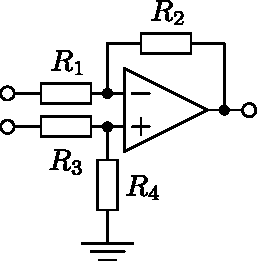
\includegraphics[scale=\schscale]{../fig/op_sub.pdf}
	\caption{Subtrahierer / Differenzverstärker}
	\label{sch:op-sub}
\end{figure}
\[ U_a = \frac{(R_1 + R_2) \cdot R_4}{(R_3 + R_4) \cdot R_1} \cdot U_{e+} 
- \frac{R_2}{R_1} \cdot U_{e-} \]
Wenn $R_1 = R_3$ und $R_2 = R_4$: 
\[ U_a = \frac{R_2}{R_1} \cdot (U_{e+} - U_{e-}) \]
Wenn $R_1 = R_2 = R_3 = R_4$: 
\[ U_a = U_{e+} - U_{e-} \]
\[ R_{e+} = R_3 + R_4 \]
\[ R_{e-} = R_1 \]
\[ R_a = 0 \]          % Subtrahierer
% coding:utf-8

%FOSAET, a LaTeX-Code for a electrical summary of basic electronics
%Copyright (C) 2013, Daniel Winz, Ervin Mazlagic

%This program is free software; you can redistribute it and/or
%modify it under the terms of the GNU General Public License
%as published by the Free Software Foundation; either version 2
%of the License, or (at your option) any later version.

%This program is distributed in the hope that it will be useful,
%but WITHOUT ANY WARRANTY; without even the implied warranty of
%MERCHANTABILITY or FITNESS FOR A PARTICULAR PURPOSE.  See the
%GNU General Public License for more details.
%----------------------------------------

\subsection{Differenzierer}
\begin{figure}[h!]
	\centering
	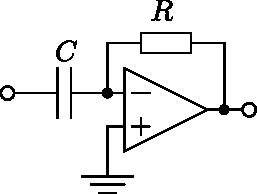
\includegraphics[scale=\schscale]{../fig/op_diff.pdf}
	\caption{Differenzierer}
	\label{sch:op-diff}
\end{figure}
\[ U_a = - R \cdot C \cdot \frac{d U_e(t)}{dt} \]
\[ X_e = \frac{1}{j \cdot \omega \cdot f \cdot C} \]
\[ R_a = 0 \]         % Differenzierer
% coding:utf-8

%FOSAET, a LaTeX-Code for a electrical summary of basic electronics
%Copyright (C) 2013, Daniel Winz, Ervin Mazlagic

%This program is free software; you can redistribute it and/or
%modify it under the terms of the GNU General Public License
%as published by the Free Software Foundation; either version 2
%of the License, or (at your option) any later version.

%This program is distributed in the hope that it will be useful,
%but WITHOUT ANY WARRANTY; without even the implied warranty of
%MERCHANTABILITY or FITNESS FOR A PARTICULAR PURPOSE.  See the
%GNU General Public License for more details.
%----------------------------------------

\subsection{Integrierer}
          % Integrierer
% coding:utf-8

%FOSAET, a LaTeX-Code for a electrical summary of basic electronics
%Copyright (C) 2013, Daniel Winz, Ervin Mazlagic

%This program is free software; you can redistribute it and/or
%modify it under the terms of the GNU General Public License
%as published by the Free Software Foundation; either version 2
%of the License, or (at your option) any later version.

%This program is distributed in the hope that it will be useful,
%but WITHOUT ANY WARRANTY; without even the implied warranty of
%MERCHANTABILITY or FITNESS FOR A PARTICULAR PURPOSE.  See the
%GNU General Public License for more details.
%----------------------------------------

\subsection{Stromquelle}
\begin{figure}[h!]
	\centering
	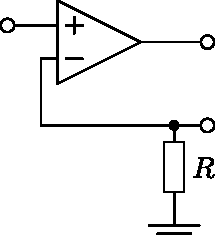
\includegraphics[scale=\schscale]{op_isource.pdf}
	\caption{Stromquelle}
	\label{sch:op-isource}
\end{figure}
\[ I_a = \frac{U_e}{R} \]
\[ R_e = \infty \]
\[ R_a = \infty \]
      % Stromquelle
% coding:utf-8

%FOSAET, a LaTeX-Code for a electrical summary of basic electronics
%Copyright (C) 2013, Daniel Winz, Ervin Mazlagic

%This program is free software; you can redistribute it and/or
%modify it under the terms of the GNU General Public License
%as published by the Free Software Foundation; either version 2
%of the License, or (at your option) any later version.

%This program is distributed in the hope that it will be useful,
%but WITHOUT ANY WARRANTY; without even the implied warranty of
%MERCHANTABILITY or FITNESS FOR A PARTICULAR PURPOSE.  See the
%GNU General Public License for more details.
%----------------------------------------

\subsection{Strom-Spannungswandler}
\begin{figure}[h!]
	\centering
	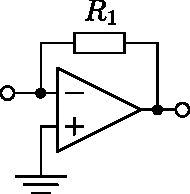
\includegraphics[scale=\schscale]{../fig/op_iu.pdf}
	\caption{Strom-Spannungswandler}
	\label{sch:op-iu}
\end{figure}
\[ V_u = - R_1 \]
\[ U_a = - I_e \cdot R_1 \]
\[ R_e = 0 \]
\[ R_a = 0 \]           % Strom-Spannungswandler
% coding:utf-8

%FOSAET, a LaTeX-Code for a electrical summary of basic electronics
%Copyright (C) 2013, Daniel Winz, Ervin Mazlagic

%This program is free software; you can redistribute it and/or
%modify it under the terms of the GNU General Public License
%as published by the Free Software Foundation; either version 2
%of the License, or (at your option) any later version.

%This program is distributed in the hope that it will be useful,
%but WITHOUT ANY WARRANTY; without even the implied warranty of
%MERCHANTABILITY or FITNESS FOR A PARTICULAR PURPOSE.  See the
%GNU General Public License for more details.
%----------------------------------------


\subsection{Frequenzgang - Realer OP}

\[ V_{UO} \cdot f_{go} = 1 \cdot f_T \]

\begin{tabular}{@{}ll}

  $V_{UO}$:	    & Openloop Versärkung DC \\
  $f_{go}$:     & Openloop Grenzfrequenz \\   
  $f_T$:        & Transitfrequenz \\
                
\end{tabular}
        % Frequenzgang
% coding:utf-8

%FOSAET, a LaTeX-Code for a electrical summary of basic electronics
%Copyright (C) 2013, Daniel Winz, Ervin Mazlagic

%This program is free software; you can redistribute it and/or
%modify it under the terms of the GNU General Public License
%as published by the Free Software Foundation; either version 2
%of the License, or (at your option) any later version.

%This program is distributed in the hope that it will be useful,
%but WITHOUT ANY WARRANTY; without even the implied warranty of
%MERCHANTABILITY or FITNESS FOR A PARTICULAR PURPOSE.  See the
%GNU General Public License for more details.
%----------------------------------------


\subsection{Verhalten am Ausgang}

Begrenzung der maximalen Ausgangsspannung durch die Slew Rate bei Sinussignal.

\[ f_{FPB} = \frac{SR}{2 \cdot \pi \cdot \^{u}_{a max} } \]

\begin{tabular}{@{}ll}

  $f_{FPB}$:	          & Full Power Bandwidth Frequenz \\
  $SR$:                   & Slew Rate (Anstiegsgeschwindigkeit) \\   
  $\^{u}_{a max}$:        & maximale Ausgangsspannung \\
                
\end{tabular}
      % Verhalten am Ausgang

% Kühlung
% coding:utf-8

%FOSAET, a LaTeX-Code for a electrical summary of basic electronics
%Copyright (C) 2013, Daniel Winz, Ervin Mazlagic

%This program is free software; you can redistribute it and/or
%modify it under the terms of the GNU General Public License
%as published by the Free Software Foundation; either version 2
%of the License, or (at your option) any later version.

%This program is distributed in the hope that it will be useful,
%but WITHOUT ANY WARRANTY; without even the implied warranty of
%MERCHANTABILITY or FITNESS FOR A PARTICULAR PURPOSE.  See the
%GNU General Public License for more details.
%----------------------------------------

\section{Thermisches Ersatzschaltbild}
\begin{figure}[h!]
  \centering
  \begin{circuitikz}[scale=1]\draw
%     (0,0) to[short, o-] (0,0)
%     (0,0) to[short, -o] (0,0)
    (0,6) to[R=$R_{th_{JC}}$, o-o] (0,4)
    (0,4) to[R=$R_{th_{CH}}$, o-o] (0,2)
    (0,2) to[R=$R_{th_{HA}}$, o-o] (0,0)
    (0.4,6) node {J}
    (0.4,4) node {C}
    (0.4,2) node {H}
    (0.4,0) node {A}
    ;
  \end{circuitikz}
  \caption{Thermisches Ersatzschaltbild}
\end{figure}
Äquivalent zu Ohmschem Gesetz: 
\[ \Delta\vartheta = R_{th} \cdot P_v \]
\[ R_{th} = \frac{\ell}{\lambda \cdot A} \]
\begin{tabular}{@{}ll}
  $J$: & Junction $\rightarrow$ Sperrschicht \\
  $C$: & Case $\rightarrow$ Gehäuse \\
  $H$: & Heatsink $\rightarrow$ Kühlkörper \\
  $A$: & Ambient $\rightarrow$ Umgebung (Achtung! Meist innerhalb Gerät) \\
  $\lambda$: & Thermische Leitfähigkeit
\end{tabular}
         % Thermisches Ersatzschaltbild